% 3

\chapter{Analisi e progettazione}

% 3.1

\section{Descrizione del problema}

Si vuole realizzare un'applicazione desktop per l'analisi di bilancio di un'azienda per l'ordine dei commercialisti della provincia di Ancona.
L'applicazione deve funzionare in tutti i vari tipi di sistema operativo, perciò il software deve essere cross-platform.
Per poter realizzare un prodotto che sia cross-platform, ossia implementato per più piattaforme di elaborazione, la scelta delle tecnologie da utilizzare è stata fondamentale.
Quando si vuole sviluppare un'applicazione desktop la prima cosa a cui si pensa è per quale sistema operativo svilupparla, quale linguaggio usare ed opzionalmente a quale base dati si ha bisogno di connettersi.
Il mondo dell'informatica intanto si sta evolvendo verso l'utilizzo di applicazioni web per la loro semplicità di distribuzione e aggiornamento, la compatibilità con ogni sistema operativo e la superfluità di un'installazione, allora perchè non sfruttare questa tecnologia?
Per questo la scelta è ricaduta su un compromesso valido, Electron.
Definita dallo slogan "Build cross platform desktop apps with Javascript, HTML, and CSS", Electron è una libreria open source sviluppata dal team di GitHub che permette di sviluppare un’applicazione desktop utilizzando le stesse tecnologie di un sito web, unendo la potenza del browser Chromium, la flessibilità di Node.js e il più grande ecosistema di librerie open source al mondo: npm. In aggiunta a tutto questo la possibilità di pacchettizzare l’applicazione per Mac, Windows, e Linux con lo stesso risultato in termini di grafica e funzionalità.

L'applicazione realizzata, nello specifico, dovrà permettere all'utente che la utilizza l'inserimento in input dei dati relativi all'Anagrafica, all'Analisi Qualitativa, dello Stato Patrimoniale e del Conto Economico di un'azienda.
Nella fase di inserimento dei valori dello Stato Patrimoniale e del Conto Economico, il sistema calcola le varie riclassificazioni dello Stato Patrimoniale (Funzionale, Finanziario o entrambi, a seconda della scelta da parte dell'utente) e del Conto Economico (al Valore Aggiunto).
L'utente deve avere la possibilità di salvare in corso d'opera il progetto e poterlo riaprire in un secondo momento.
Inoltre, va implementata una funzione che permette la stampa in un file pdf del progetto.


% 3.2

\section{Analisi dei requisiti}

Al fine di esporre i requisiti in maniera rigorosa, verrà adottata la notazione MoSCoW, la quale fa uso delle seguenti etichette:
\begin{itemize}
\item Must Have: sottolinea un requisito di fondamentale importanza per il funzionamento del sistema;
\item Should Have: indica un requisito importante ma non essenziale per il funzionamento del sistema;
\item Could Have (o Nice to Have): indica un requisito non importante come i precedenti e volto principalmente a migliorare la soddisfazione del cliente.
\item Won’t Have: requisiti che non devono essere implementati (negazione di una funzione).
\end{itemize}

% 3.2.1

\newpage

\subsection{Requisiti funzionali}
I requisiti funzionali descrivono le funzionalità del sistema software, in termini di servizi che il sistema software deve fornire, di come il sistema software reagisce a specifici tipi di input e di come si comporta in situazioni particolari.

\begin{table}[H]
    \footnotesize
    \centering
    \begin{tabulary}{0.9\textwidth}{|L|L|c|}
        \hline
        ID & Descrizione & MoSCoW \\
        \hline\hline
        1 & Il programma deve permettere l'inserimento e la visualizzazione dei dati dell'azienda di cui si vuole analizzare il bilancio & Must have \\
        \hline
        2 & Il programma deve permettere all'utente il salvataggio del progetto & Must have \\
        \hline
        3 & Il programma deve permettere all'utente l'apertura di un progetto salvato in precedenza & Must have \\
        \hline
        4 & Il programma deve permettere all'utente di scegliere quale tipo di riclassificazione per lo stato patrimoniale utilizzare & Must have \\
        \hline
        5 & Il programma deve calcolare le riclassificazioni sia per lo stato patrimoniale che per il conto economico & Must have \\
        \hline
        6 & Il programma deve permettere all'utente di poter inserire l'annualità di riferimento dell'analisi & Should have \\
        \hline
        7 & Il programma deve permettere all'utente di poter stampare in un formato pdf del progetto & Should have \\
        \hline
        8 & Il programma deve calcolare in automatico il forecast per le annualità previste dall'utente & Could have \\
        \hline
    \end{tabulary}
    \caption{Requisiti funzionali}
\end{table}

% 3.2.2

\newpage

\subsection{Requisiti non funzionali}
Descrivono le proprietà del sistema software in relazione a determinati servizi o funzioni e possono anche essere relativi al processo:
\begin{itemize}
\item Caratteristiche di efficienza, affidabilità, safety, ecc.
\item Caratteristiche del processo di sviluppo (standard di processo, linguaggi di programmazione, metodi di sviluppo, ecc.
\item Caratteristiche esterne (interoperabilità con sistemi di altre organizzazioni, vincoli legislativi, ecc.)
\end{itemize}

\begin{table}[H]
    \footnotesize
    \centering
    \begin{tabulary}{0.9\textwidth}{|L|L|c|}
        \hline
        ID & Descrizione & MoSCoW \\
        \hline\hline
        1 & Il programma deve essere sviluppato per tutte le piattaforme di elaborazione & Must have \\
        \hline
        2 & Il programma dovrebbe controllare i formati di immissione dei dati nella maschera di input & Should have \\
        \hline
        3 & L'avvio e in particolar modo la ricezione dell'input da parte dell'utente, dovrebbe essere veloce & Should have \\
        \hline
        4 & Il programma deve calcolare ina maniera veloce le riclassificazioni & Should have \\
        \hline
        5 & Il programma può essere adattabile alle differenti risoluzioni dello schermo (responsive) & Could have \\
        \hline
    \end{tabulary}
    \caption{Requisiti non funzionali}
\end{table}

% 3.3

\newpage

\section{Use case diagram}

Gli Use Case Diagrams descrivono il comportamento funzionale del sistema, come visto dall’utente. Sono diagrammi di facile interpretazione dove abbiamo uno o più attori che possono attivare diverse funzioni/servizi all'interno di uno o più sistemi. Servono a riepilogare i dettagli degli utenti del sistema (noti anche come attori) e le loro interazioni con il sistema.

\begin{figure}[H]
    \centering
    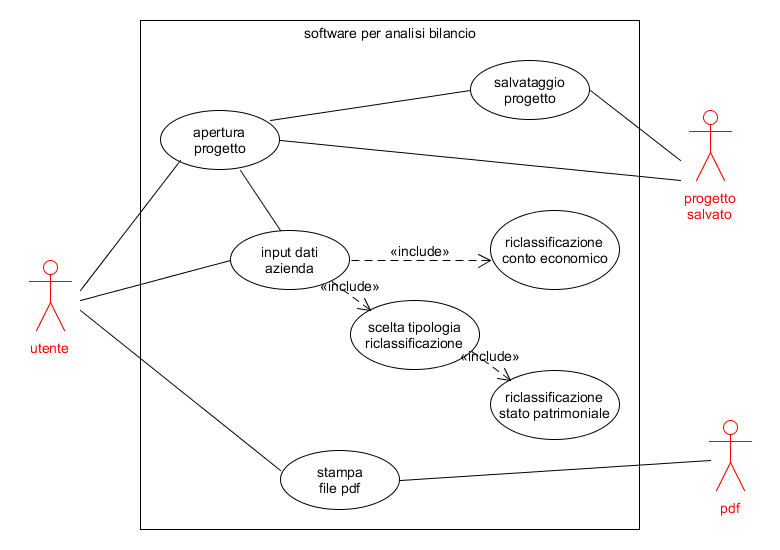
\includegraphics[scale=0.5]{use-case-diagram.png}
    \caption{UML Use Case Diagram}
    \label{fig:UseCase1}
\end{figure}

Nel diagramma in figura  ~\ref{fig:UseCase1} abbiamo tre attori, l'utente che inserisce i dati dell'azienda, il file contenente il progetto salvato e il file pdf generato dal software.
I casi d'uso talvolta includono più passaggi al loro interno, in quei casi è indicata una freccia "include", come nel caso del "input dati azienda" che include "scelta tipologia riclassificazione" che a sua volta include "riclassificazione stato patrimoniale".

% 3.4

\newpage

\section{Activity diagram}

L'Activity Diagram è un diagramma che definisce le attività da svolgere per realizzare una data funzionalità ed è spesso utilizzato come modello complementare dello Use Case Diagram.

\begin{figure}[H]
    \centering
    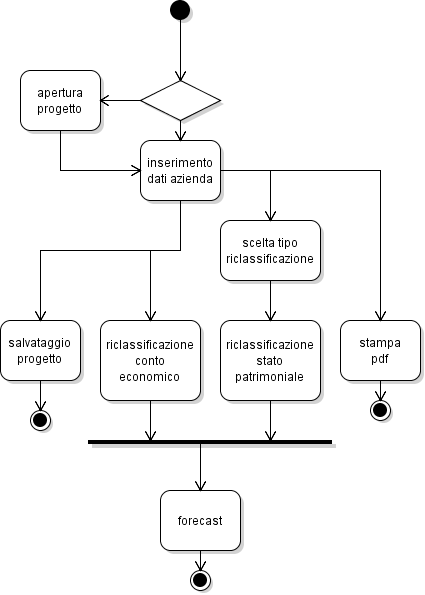
\includegraphics[scale=0.6]{activity-diagram.png}
    \caption{UML Activity Diagram}
    \label{fig:ActivityDiagram1}
\end{figure}

Nella figura ~\ref{fig:ActivityDiagram1} vediamo descritto il software come nello Use Case precedente, ma dal punto di vista delle attività da svolgere in sequenza per raggiungere un certo risultato.
Il diagramma si legge a partire dal pallino in alto, detto nodo iniziale, seguono le azioni indicate dai rettangoli.
I rombi indicano le decisioni, cioè le diverse direzioni che può prendere il flusso a seguito di certe condizioni o scelte, ad esempio all'avvio del software se si vuole aprire un progetto salvato precedentemente o inserire i dati per un nuovo progetto.
Un altro elemento dell'activity diagram è la "join", che indica che per passare all'azione successiva devono essere completate tutte le azioni in ingresso, come ad esempio per il calcolo del forecast, che avviene una volta inseriti i dati e quindi calcolate le riclassificazioni dello
stato patrimoniale e del conto economico.

% 3.5

\newpage

\section{Sequence diagram}

Il sequence diagram è uno strumento di modellazione visuale che mette in evidenza come i vari componenti di un sistema interagiscono tra di loro in relazione al tempo.

\begin{figure}[H]
    \centering
    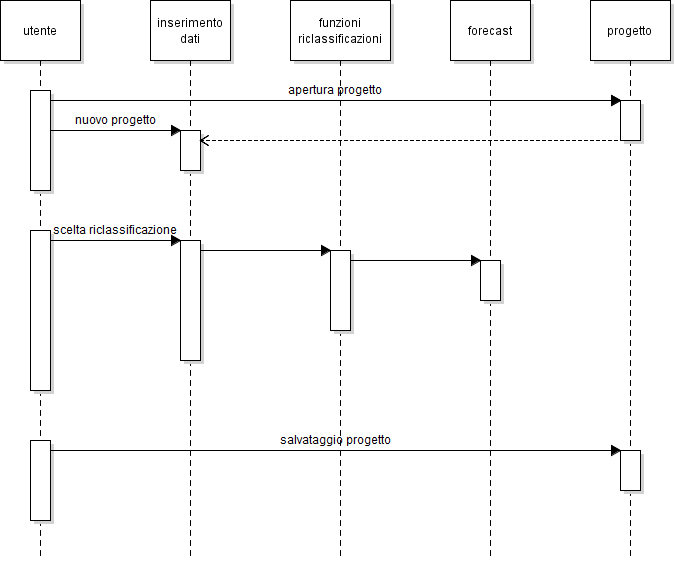
\includegraphics[scale=0.6]{sequence-diagram.png}
    \caption{UML Sequence Diagram}
    \label{fig:SequenceDiagram}
\end{figure}

Nella figura ~\ref{fig:SequenceDiagram} vediamo descritto il flusso iniziale del software che inizia con la scelta da parte dell'utente di creazione di un nuovo progetto o di aprire un progetto salvato precedentemente e termina con il salvataggio dello stesso dopo aver calcolato tutte le riclassificazioni.
I componenti del diagramma sono l'utente, la form che permette l'input dei dati, le funzioni per le riclassificazioni, la funzione del forecast e il progetto salvato esternamente.
Nella fase di inserimento dei dati da parte dell'utente, il sistema calcola le varie riclassificazioni, tendendo conto della scelta dell'utente della tipologia scelta per lo Stato Patrimoniale, e mette tutto a disposizione per il salvataggio dei dati e per la stampa del pdf.